

\section{Estratégias de Jogos}
\begin{frame}

    \frametitle{Teoria de Jogos}
    \begin{itemize}
    \pause
      \item 
\pause
      \item cap 3
    
    \end{itemize}
\end{frame}


\section{Coordenação}
\begin{frame}

    \frametitle{Coordenação}
    \begin{itemize}
    \pause
      \item 
\pause
      \item cap 4
    
    \end{itemize}
\end{frame}

\subsection{Exemplos de Coordenação SMAs}

\begin{frame}
\frametitle{Exemplo de Coordenação SMAs}

\begin{figure}[!ht]
\centering
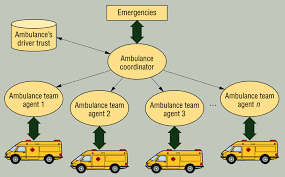
\includegraphics[height =.6\textheight,width=.7\textwidth]{figuras/coordenacao_agentes01.png}
\caption{Coordenação de agentes $\equiv $   SMA}
%\label{ag_01}
\end{figure}
 \end{frame}





\begin{frame}
\frametitle{Exemplo de Coordenação SMAs}

\begin{figure}[!ht]
\centering
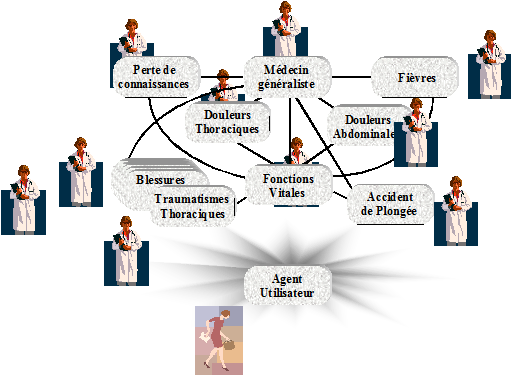
\includegraphics[height =.6\textheight,width=.7\textwidth]{figuras/coordenacao_agentes02.png}
\caption{Coordenação de agentes $\equiv $   SMA}
%\label{ag_01}
\end{figure}
 
\end{frame}

\section{Teoria de Jogos Aplicado a SMA}
\begin{frame}

    \frametitle{Teoria de Jogos Aplicado a SMA}
    \begin{itemize}
    \pause
      \item $\prod^{n}_{x=1} \neq  \prod_{x=1}^{n+1}$
      \item  \url{https://www.codecogs.com/latex/eqneditor.php}
      \item \url{http://www.hostmath.com/}
      

      \pause
      \item cap 6
    
    \end{itemize}
\end{frame}



